% Introduction chapter.
%
% Developed for my Master Thesis at Maastricht University.
% Based on Eugenio Senes's template at the University of Torino.
%
% By Joeri Hermans (joeri@joerihermans.com)
%
% Released under an MIT license. Share, modify and enjoy, but quote the author!

\chapter{Introduction}
\label{chapter:introduction}

In this chapter we introduce the main concept, and problems surrounding the parallization of gradient descent. We familliarize the reader with the topic and some notation by providing some context why someone would like to apply said technique. Furthermore, in Section~\ref{sec:problem_statement}, we summarize the problem statement and provide several research questions which will guide the research in this work. Finally, we conclude this chapter in Section~\ref{sec:thesis_outline} with a brief outline of the thesis.

\section{Motivation}
\label{sec:motivation}

In recent years it has been shown that being able to train large and deep neural networks result in state-of-the-art performance~\cite{wu2016google, dean2012large}, especially regarding unsupervised feature learning and image recognition. However, consider the required time, and cost of the infrastructure that would be required in order to train such a large model in a reasonable amount of time. Furthermore, it is not only the training time and cost of the infrastructure which need to be taken into consideration, but also the volume of the data. The amount of information that will be gathered will be an increasing important factor in the next few years. Not only with respect to big technology companies and government organizations, but also scientific surveys with limited budgets. These scientific surveys will generate more experimental data than ever~\cite{hllhcdesignreport, ivezic2008lsst}, and will have to process and analyze that data. To solve the problem of increased computational workloads and budget freezes, the High Energy Physics (HEP) community is exploring and researching machine learning approaches to fit physics problems~\cite{bian2016recent, de2017learning, louppe2016learning} with the intention to improve detection quality, or reduce computational constraints.\\

However, the sheer size of these datasets severly impacts the training time of the models. In order to resolve this issue, one could sample some representative subset of the data in order to reduce the training time. The disadvantage of this approach is that is possible that some ``diverse`` instances, i.e., data points, do not appear in the final training set. This is especially a problem in Deep Learning, where models usually benifit from having access to a lot of training data due to the high dimensionality of the parametrization~\cite{dean2012large}. In order to resolve this issue, Dean et al.~\cite{dean2012large} introduce two new paradigms to decrease the training time in the prescense of a large dataset and a high dimensionality of the parametrization. The two paradigms, \emph{Model Parallelism}, briefly discussed in Section~\ref{sec:intro_model_parallelism}, and \emph{Data Parallelism}, discussed in Section~\ref{sec:intro_data_parallelism}, are inherently different ways of decreasing the training time of a model.\\

The first paradigm, \emph{Model Parallelism}, is the intuitively most straightforward one since it deals with the parallelization of the computations within a \emph{single} model, i.e., how to parallelize the computations of a single model over multiple machines, or multiple processes. The second paradigm, which will be the main focus of this thesis, is \emph{Data Parallelism}. As stated above, the main concept of Data Parallelism will be discussed in detail in Section~\ref{sec:intro_data_parallelism}. However, for completion, think of Data Parallelism as a technique to \emph{parallelize gradient descent}. This is done by allocating $n$ processes over possibly $n$ different machines, and splitting the training set into $n$ \emph{partitions}, or \emph{shards}. For further convenience, we will call such a process a \emph{worker}. In the next step, we assign a single distinct partition to a worker. Meaning, the worker will not be able to fetch training data from other partitions since those have been assigned to different workers. The goal of these workers is to work together, and optimize the parameters of a central model. A lot of different distributed optimization schemes have been suggested in recent years~\cite{zhang2015deep, dean2012large, hadjis2016omnivore, ??}. Most of the recent contributions try to push the limits of (asynchronous) Data Parallelism by simply \emph{annealing} the gradients with respect to some hyperparameter without giving a sound theoretical argument why the annealing should happen in the first place.\\

Recently, new theoretical work supported by experimental evidence was introduced by Mitliagkas et al.~\cite{implicitmomentum}. We will discuss this work in detail, and provide some supporting experimental evidence in Section~\ref{sec:implicit_momentum}.

\section{Model Parallelism}
\label{sec:intro_model_parallelism}

\section{Data Parallelism}
\label{sec:intro_data_parallelism}

\begin{figure}[H]
  \centering
  % Define database shape.
  \def\database at (#1,#2){
    \draw (#1,#2) ellipse (0.5 and 0.15);
    \draw (#1 - 0.5, #2) -- (#1 - 0.5, #2 - 1);
    \draw (#1 + 0.5, #2) -- (#1 + 0.5, #2 - 1);
    \draw (#1 - 0.5, #2 - 1/3) arc (180:360:0.5 and 0.15);
    \draw (#1 - 0.5, #2 - 2/3) arc (180:360:0.5 and 0.15);
    \draw (#1 - 0.5, #2 - 1) arc (180:360:0.5 and 0.15);
  }
  % Define datashard shape.
  \def\datashard at (#1,#2){
    \draw (#1,#2) ellipse (0.5 and 0.15);
    \draw (#1 - 0.5, #2) -- (#1 - 0.5, #2 - 1/3);
    \draw (#1 + 0.5, #2) -- (#1 + 0.5, #2 - 1/3);
    \draw (#1 - 0.5, #2 - 1/3) arc (180:360:0.5 and 0.15);
  }
  % Define the neural network shape.
  \def\neuralnet at (#1,#2){
    % Draw node bounding box.
    \draw[rounded corners=3pt] (#1 - 0.7,#2 + 0.5) rectangle ++(1.4,-0.95);
    % Draw fully connected lines.
    \draw[gray] (#1 + 0.25,#2) -- (#1 - 0.375, #2 + 0.25);
    \draw[gray] (#1 + 0.25,#2) -- (#1 - 0.125, #2 + 0.25);
    \draw[gray] (#1 + 0.25,#2) -- (#1 + 0.125, #2 + 0.25);
    \draw[gray] (#1 + 0.25,#2) -- (#1 + 0.375, #2 + 0.25);
    \draw[gray] (#1 + 0.5,#2) -- (#1 - 0.375, #2 + 0.25);
    \draw[gray] (#1 + 0.5,#2) -- (#1 - 0.125, #2 + 0.25);
    \draw[gray] (#1 + 0.5,#2) -- (#1 + 0.125, #2 + 0.25);
    \draw[gray] (#1 + 0.5,#2) -- (#1 + 0.375, #2 + 0.25);
    \draw[gray] (#1,#2) -- (#1 - 0.375, #2 + 0.25);
    \draw[gray] (#1,#2) -- (#1 - 0.125, #2 + 0.25);
    \draw[gray] (#1,#2) -- (#1 + 0.125, #2 + 0.25);
    \draw[gray] (#1,#2) -- (#1 + 0.375, #2 + 0.25);
    \draw[gray] (#1 - 0.25,#2) -- (#1 - 0.375, #2 + 0.25);
    \draw[gray] (#1 - 0.25,#2) -- (#1 - 0.125, #2 + 0.25);
    \draw[gray] (#1 - 0.25,#2) -- (#1 + 0.125, #2 + 0.25);
    \draw[gray] (#1 - 0.25,#2) -- (#1 + 0.375, #2 + 0.25);
    \draw[gray] (#1 - 0.5,#2) -- (#1 - 0.375, #2 + 0.25);
    \draw[gray] (#1 - 0.5,#2) -- (#1 - 0.125, #2 + 0.25);
    \draw[gray] (#1 - 0.5,#2) -- (#1 + 0.125, #2 + 0.25);
    \draw[gray] (#1 - 0.5,#2) -- (#1 + 0.375, #2 + 0.25);
    \draw[gray] (#1 + 0.25,#2) -- (#1 + 0.125, #2 - 0.25);
    \draw[gray] (#1 + 0.25,#2) -- (#1 - 0.125, #2 - 0.25);
    \draw[gray] (#1 + 0.5,#2) -- (#1 + 0.125, #2 - 0.25);
    \draw[gray] (#1 + 0.5,#2) -- (#1 - 0.125, #2 - 0.25);
    \draw[gray] (#1,#2) -- (#1 + 0.125, #2 - 0.25);
    \draw[gray] (#1,#2) -- (#1 - 0.125, #2 - 0.25);
    \draw[gray] (#1 - 0.25,#2) -- (#1 + 0.125, #2 - 0.25);
    \draw[gray] (#1 - 0.25,#2) -- (#1 - 0.125, #2 - 0.25);
    \draw[gray] (#1 - 0.5,#2) -- (#1 + 0.125, #2 - 0.25);
    \draw[gray] (#1 - 0.5,#2) -- (#1 - 0.125, #2 - 0.25);
    % Define input layer.
    \draw[fill=white] (#1 - 0.375,#2 + 0.25) circle (1pt);
    \draw[fill=white] (#1 - 0.125,#2 + 0.25) circle (1pt);
    \draw[fill=white] (#1 + 0.125,#2 + 0.25) circle (1pt);
    \draw[fill=white] (#1 + 0.375,#2 + 0.25) circle (1pt);
    % Define hidden layer.
    \draw[fill=white] (#1 - 0.5,#2) circle (1pt);
    \draw[fill=white] (#1 - 0.25,#2) circle (1pt);
    \draw[fill=white] (#1,#2) circle (1pt);
    \draw[fill=white] (#1 + 0.25,#2) circle (1pt);
    \draw[fill=white] (#1 + 0.5,#2) circle (1pt);
    % Define output layer.
    \draw[fill=white] (#1 - 0.125,#2 - 0.25) circle (1pt);
    \draw[fill=white] (#1 + 0.125,#2 - 0.25) circle (1pt);
  }
  \def\neuralnetclean at (#1,#2){
    \draw[gray] (#1 + 0.25,#2) -- (#1 - 0.375, #2 + 0.25);
    \draw[gray] (#1 + 0.25,#2) -- (#1 - 0.125, #2 + 0.25);
    \draw[gray] (#1 + 0.25,#2) -- (#1 + 0.125, #2 + 0.25);
    \draw[gray] (#1 + 0.25,#2) -- (#1 + 0.375, #2 + 0.25);
    \draw[gray] (#1 + 0.5,#2) -- (#1 - 0.375, #2 + 0.25);
    \draw[gray] (#1 + 0.5,#2) -- (#1 - 0.125, #2 + 0.25);
    \draw[gray] (#1 + 0.5,#2) -- (#1 + 0.125, #2 + 0.25);
    \draw[gray] (#1 + 0.5,#2) -- (#1 + 0.375, #2 + 0.25);
    \draw[gray] (#1,#2) -- (#1 - 0.375, #2 + 0.25);
    \draw[gray] (#1,#2) -- (#1 - 0.125, #2 + 0.25);
    \draw[gray] (#1,#2) -- (#1 + 0.125, #2 + 0.25);
    \draw[gray] (#1,#2) -- (#1 + 0.375, #2 + 0.25);
    \draw[gray] (#1 - 0.25,#2) -- (#1 - 0.375, #2 + 0.25);
    \draw[gray] (#1 - 0.25,#2) -- (#1 - 0.125, #2 + 0.25);
    \draw[gray] (#1 - 0.25,#2) -- (#1 + 0.125, #2 + 0.25);
    \draw[gray] (#1 - 0.25,#2) -- (#1 + 0.375, #2 + 0.25);
    \draw[gray] (#1 - 0.5,#2) -- (#1 - 0.375, #2 + 0.25);
    \draw[gray] (#1 - 0.5,#2) -- (#1 - 0.125, #2 + 0.25);
    \draw[gray] (#1 - 0.5,#2) -- (#1 + 0.125, #2 + 0.25);
    \draw[gray] (#1 - 0.5,#2) -- (#1 + 0.375, #2 + 0.25);
    \draw[gray] (#1 + 0.25,#2) -- (#1 + 0.125, #2 - 0.25);
    \draw[gray] (#1 + 0.25,#2) -- (#1 - 0.125, #2 - 0.25);
    \draw[gray] (#1 + 0.5,#2) -- (#1 + 0.125, #2 - 0.25);
    \draw[gray] (#1 + 0.5,#2) -- (#1 - 0.125, #2 - 0.25);
    \draw[gray] (#1,#2) -- (#1 + 0.125, #2 - 0.25);
    \draw[gray] (#1,#2) -- (#1 - 0.125, #2 - 0.25);
    \draw[gray] (#1 - 0.25,#2) -- (#1 + 0.125, #2 - 0.25);
    \draw[gray] (#1 - 0.25,#2) -- (#1 - 0.125, #2 - 0.25);
    \draw[gray] (#1 - 0.5,#2) -- (#1 + 0.125, #2 - 0.25);
    \draw[gray] (#1 - 0.5,#2) -- (#1 - 0.125, #2 - 0.25);
    % Define input layer.
    \draw[fill=white] (#1 - 0.375,#2 + 0.25) circle (1pt);
    \draw[fill=white] (#1 - 0.125,#2 + 0.25) circle (1pt);
    \draw[fill=white] (#1 + 0.125,#2 + 0.25) circle (1pt);
    \draw[fill=white] (#1 + 0.375,#2 + 0.25) circle (1pt);
    % Define hidden layer.
    \draw[fill=white] (#1 - 0.5,#2) circle (1pt);
    \draw[fill=white] (#1 - 0.25,#2) circle (1pt);
    \draw[fill=white] (#1,#2) circle (1pt);
    \draw[fill=white] (#1 + 0.25,#2) circle (1pt);
    \draw[fill=white] (#1 + 0.5,#2) circle (1pt);
    % Define output layer.
    \draw[fill=white] (#1 - 0.125,#2 - 0.25) circle (1pt);
    \draw[fill=white] (#1 + 0.125,#2 - 0.25) circle (1pt);
  }
  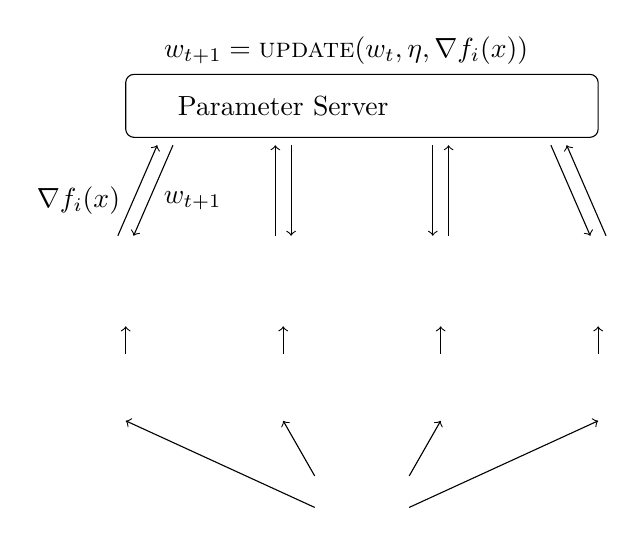
\begin{tikzpicture}
    \database at (0,0);
    \draw[->] (-0.6,-0.5) -- (-3, 0.6);
    \draw[->] (-0.6,-0.1) -- (-1, 0.6);
    \draw[->] (0.6,-0.1) -- (1, 0.6);
    \draw[->] (0.6,-0.5) -- (3, 0.6);
    \datashard at (-3,1.2)
    \datashard at (-1,1.2);
    \datashard at (1,1.2);
    \datashard at (3,1.2);
    \draw[->] (-3, 1.45) -- (-3, 1.8);
    \draw[->] (-1, 1.45) -- (-1, 1.8);
    \draw[->] (1, 1.45) -- (1, 1.8);
    \draw[->] (3, 1.45) -- (3, 1.8);
    \neuralnet at (3,2.35);
    \neuralnet at (1,2.35);
    \neuralnet at (-1,2.35);
    \neuralnet at (-3,2.35);
    % Draw the parameter server.
    \draw[rounded corners=3pt] (-3, 5) rectangle ++(6,-0.8);
    \node (pslabel) at (-1, 4.6) {Parameter Server};
    \node (psequation) at (-0.2, 5.3) {$w_{t+1} = \textsc{update}(w_t, \eta, \nabla f_i(x))$};
    % Draw the lines.
    \neuralnetclean at (1.8, 4.6);
    \draw[->] (-3.1, 2.95) -- (-2.6, 4.1);
    \draw[<-] (-2.9, 2.95) -- (-2.4, 4.1);
    \draw[->] (-1.1, 2.95) -- (-1.1, 4.1);
    \draw[<-] (-0.9, 2.95) -- (-0.9, 4.1);
    \draw[->] (1.1, 2.95) -- (1.1, 4.1);
    \draw[<-] (0.9, 2.95) -- (0.9, 4.1);
    \draw[->] (3.1, 2.95) -- (2.6, 4.1);
    \draw[<-] (2.9, 2.95) -- (2.4, 4.1);
    % Draw the labels.
    \node (commit) at (-2.15, 3.4) {$w_{t+1}$};
    \node (pull) at (-3.6, 3.4) {$\nabla f_i(x)$};
    % More labels.
  \end{tikzpicture}
  \caption{Schematic representation of a data parallel approach. In this methodology we spawn $n$ workers (not necessarily on different machines), and assign a data shard (partition) of the dataset to every worker. Using this data shard, a worker $i$ will iterate through all mini-batches to produce a gradient, $\nabla f_i(x)$, for every mini-batch $x$. Next, $\nabla f_i(x)$ is send to the parameter server, which will incorperate the gradient using an~\textsc{update} mechanism.}
  \label{fig:introduction_data_parallelism_schematic}
\end{figure}

\section{Problem Statement}
\label{sec:problem_statement}

\section{Thesis Outline}
\label{sec:thesis_outline}
